\section{Liczniki asynchroniczne}

\subsection{Zadanie}

Zrealizować licznik \textbf{asynchroniczny mod 4/13}

\subsection{komentarz}

Licznik asynchroniczny różni się od synchronicznego tym że tylko wejście zegarowe pierwszego przerzutnika jest podpięte do zegara. Wejście CLK każdego kolejnego flip flopa podpięte jest pod wyjście poprzedniego. Jeżeli licznik ma liczyć w przód to podpinamy zegar do zanegowanego wyjścia a jeśli w tył to do zwykłego Q.

\subsection{Tablica prawdy}

\begin{figure}[h!]
    \centering
    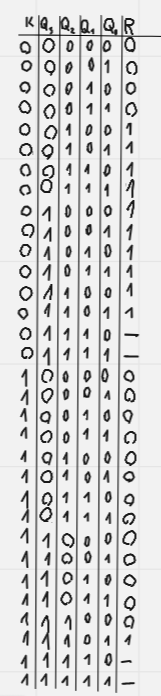
\includegraphics[width = .2\textwidth]{images/async/async_t.png}
    \caption{Tablica prawdy}
    \label{fig:my_label}
\end{figure}

\newpage

Syntezę licznika zaczynamy od rozpisania tablicy prawdy, część miejsc w tablicy jest zaznaczona jako stany nieistotne, bo nasz licznik nigdy do nich nie dotrze. Taki zapis może ułatwić nam robotę podczas liczenia siatek. Skoro licznik liczy maksymalnie do 13 no to bez sensu jest zapisywanie zer dla 14, 15 i 16 skoro i tak układ się zresetuje na trzynastce. Dodatkowo warto zauważyć że gdy licznik jest ustawiony na mod 4 to wszystkie wartości powyżej 4 też oznaczają reset, to podejście pozwala uniknąć sytuację gdy jakiś gagatek postanowi przełączyć licznik z mod 13 na mod 4 w momencie gdy stan licznika pokazuje np. 8.

\subsection{Siatka Karnaugh}

\begin{figure}[h!]
    \centering
    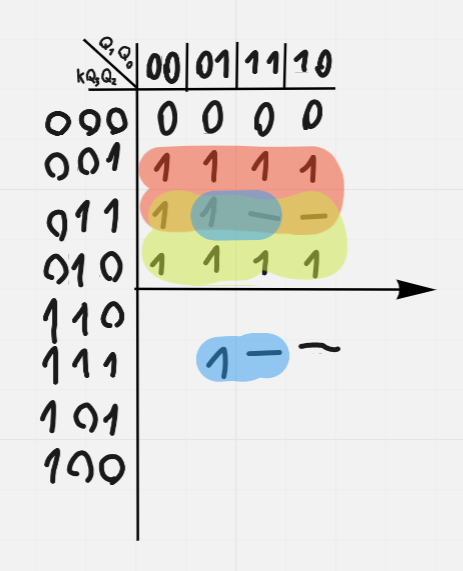
\includegraphics[width = .3\textwidth]{images/async/async_k.png}
    \caption{Siatka Karnaugh}
    \label{fig:my_label}
\end{figure}

Z tabeli robimy prostą siateczkę.

\subsection{Funkcja resetu}

\begin{figure}[h!]
    \centering
    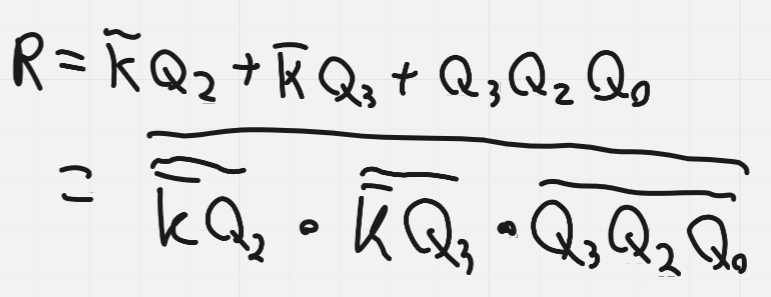
\includegraphics[width = 9cm]{images/async/async_e.png}
    \caption{Funkcja resetu}
    \label{fig:my_label}
\end{figure}

Funkcja, która wyszła z siatki została przekształcona by można było ją zbudować tylko na NANDach i negacjach.

\newpage

\subsection{Schemat układu}

\begin{figure}[h!]
    \centering
    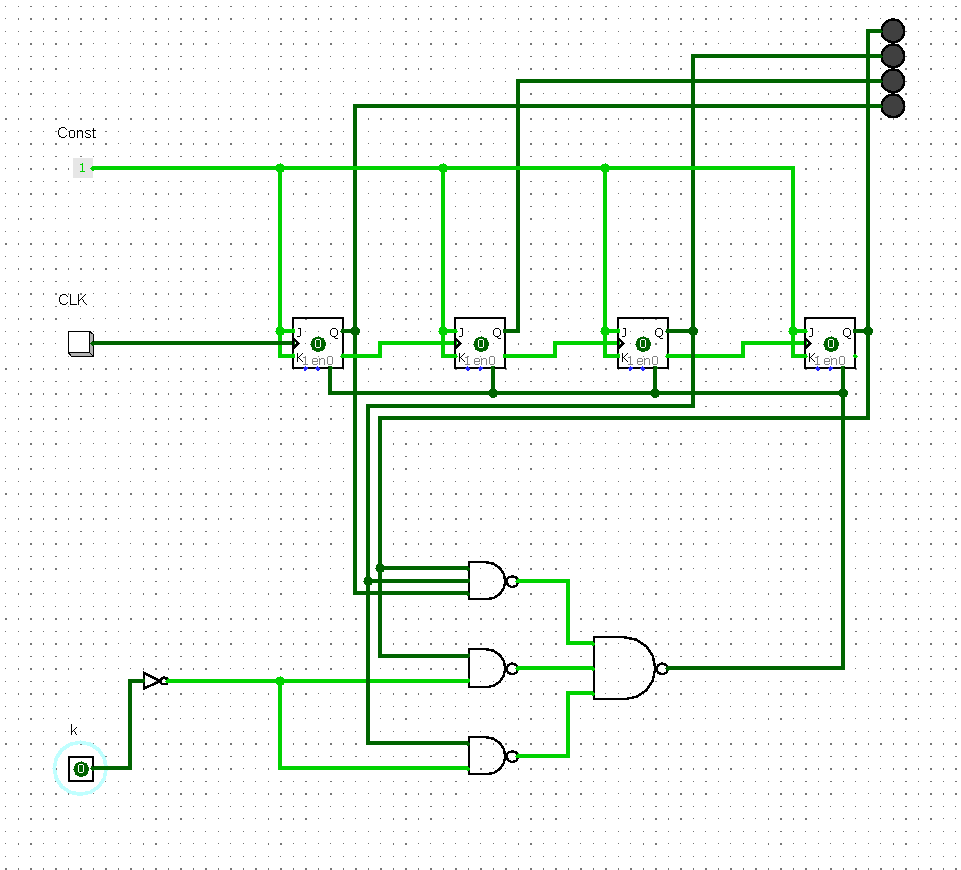
\includegraphics[width = 12cm]{images/async/async_l.png}
    \caption{Schemat układu}
    \label{fig:my_label}
\end{figure}

\newpage